\documentclass{article} % For LaTeX2e
\usepackage{CJKutf8}
\usepackage{url}
\usepackage{graphicx}
\usepackage{amsmath}
\usepackage{amsthm}
\usepackage{mathtools}
\usepackage{MnSymbol}
\usepackage{indentfirst}
\usepackage{subfigure}
\setlength{\parindent}{2em}
\usepackage{algpseudocode}
\usepackage{algorithm}
\usepackage{listings}
\usepackage{textcomp}  % \textcelsius
\usepackage{tikz}
\title{密码学基础研讨课 实验报告}
\author{秦嗣量, 2018K8009970004}
\usepackage{geometry}
\geometry{left=2.5cm,right=2.5cm,top=2.5cm,bottom=2.5cm}

\newcommand{\fix}{\marginpar{FIX}}
\newcommand{\new}{\marginpar{NEW}}

\newtheorem{theorem}{Theorem}
\newtheorem{defn}{Definition}

\begin{document}
\begin{CJK}{UTF8}{gbsn}
\maketitle
\section{实验内容}
用三种不同的方式实现AES-128-ECB加密算法,并测量各种实现的效率。

在此基础上,利用Qt框架提供较为清晰的图形界面,便于直观的检验算法的正确性、更改测试等配置操作,且使得该作品能够直接用于文件的加解密操作中。可方便的加载密钥和明文密文等,并实现加解密操作。

利用标准测试向量验证各种实现的正确性,且在试验中各种实现的结果能够相互验证。
\section{实现方法}
\subsection{基类}
将AES加密算法中共性的部分提取出来作为基类,提供统一的接口,底层实现面向该接口编程。此处设计参考了AES-NI指令集的设计。对于每个\textbf{128 bits block}的加密,对象内部维护一个\textbf{state},通过更新该成员属性实现加密过程。

\begin{description}
  \item[密钥扩展] 初始化对象时利用提供的参数进行密钥扩展,待后续加解密过程中使用。
  \item[加密] 利用\textbf{xorsi}函数执行初始的密钥加操作,然后利用\textbf{encsi}函数执行9轮,最后一轮使用\textbf{encsilast}。
  \item[解密] 利用\textbf{xorsi}函数执行初始的密钥加操作,然后利用\textbf{decsi}函数执行9轮,最后一轮使用\textbf{decsilast}。
  \item[设置状态] 利用传入的字符串初始化对象内部状态。
  \item[获取结果] 将内部状态作为字符串导出。
\end{description}

在这样的框架下,各种不同实现的区别仅在于不同内部状态的表示和每个单步操作的实现方式。
\subsection{一般实现}
逐一实现\textbf{sub\_bytes}, \textbf{shift\_rows}, \textbf{mix\_columns}, \textbf{add\_round\_key}等操作及其逆变换,并拼接以实现上述定义的接口。
\subsection{查表法实现}
\textbf{sub\_bytes}操作后还存在\textbf{mix\_columns},需要计算有限域上的矩阵乘法,通过预先计算S盒中的元素乘法运算的结果,可以将各轮变换过程转化为简单的查表、移位和异或操作的组合。可预先计算如下结果:
\begin{itemize}
  \item Te0[x] = S [x].[02, 01, 01, 03];
\item Te1[x] = S [x].[03, 02, 01, 01];
\item Te2[x] = S [x].[01, 03, 02, 01];
\item Te3[x] = S [x].[01, 01, 03, 02];
\item Te4[x] = S [x].[01, 01, 01, 01];

\item Td0[x] = Si[x].[0e, 09, 0d, 0b];
\item Td1[x] = Si[x].[0b, 0e, 09, 0d];
\item Td2[x] = Si[x].[0d, 0b, 0e, 09];
\item Td3[x] = Si[x].[09, 0d, 0b, 0e];
\item Td4[x] = Si[x].[01, 01, 01, 01];
\end{itemize}

利用上述几张表加速最终的加密过程。

\subsection{AES-NI实现}
利用AES-NI指令实现,该指令集中存在与基类中接口一一对应的函数,直接调用即可。
\section{环境配置}
\begin{enumerate}
  \item 操作系统:Manjaro Linux (Kernel Version 5.4)
  \item IDE: Qt Creator
  \item 编译器:gcc 9.3
\end{enumerate}

\section{测试原理}
给定密钥,设定明文长度,采用随机数发生器随机生成指定长度到明文。利用gcc提供的rdstc函数获取当前时间(精确到时钟周期),然后开始执行加密操作,加密完成后再次获取当前时间。求二者差值即可得到完成加密所需的总的时钟周期数。用该数据除以明文长度,即可到加密速度。
\[
Cycle Per Bytes = \frac{Cycles}{PlainTextLength} = \frac{EndTime - StartTime}{PlainTextLength}
\]

\section{测试结果}
在Debug和Release两种版本下,测试程序表现出了不同的行为:在Debug版本中,各种实现在效率上存在明显差距,AES\_NI实现 $>$ 查表实现 $>$ 一般实现,而在Release版本中经过编译优化之后的各种实现的效率基本处于同一量级。
\begin{figure}[H]
	\centering
	\label{Test}
	\subfigure[Debug] {
	\label{Debug Test}
	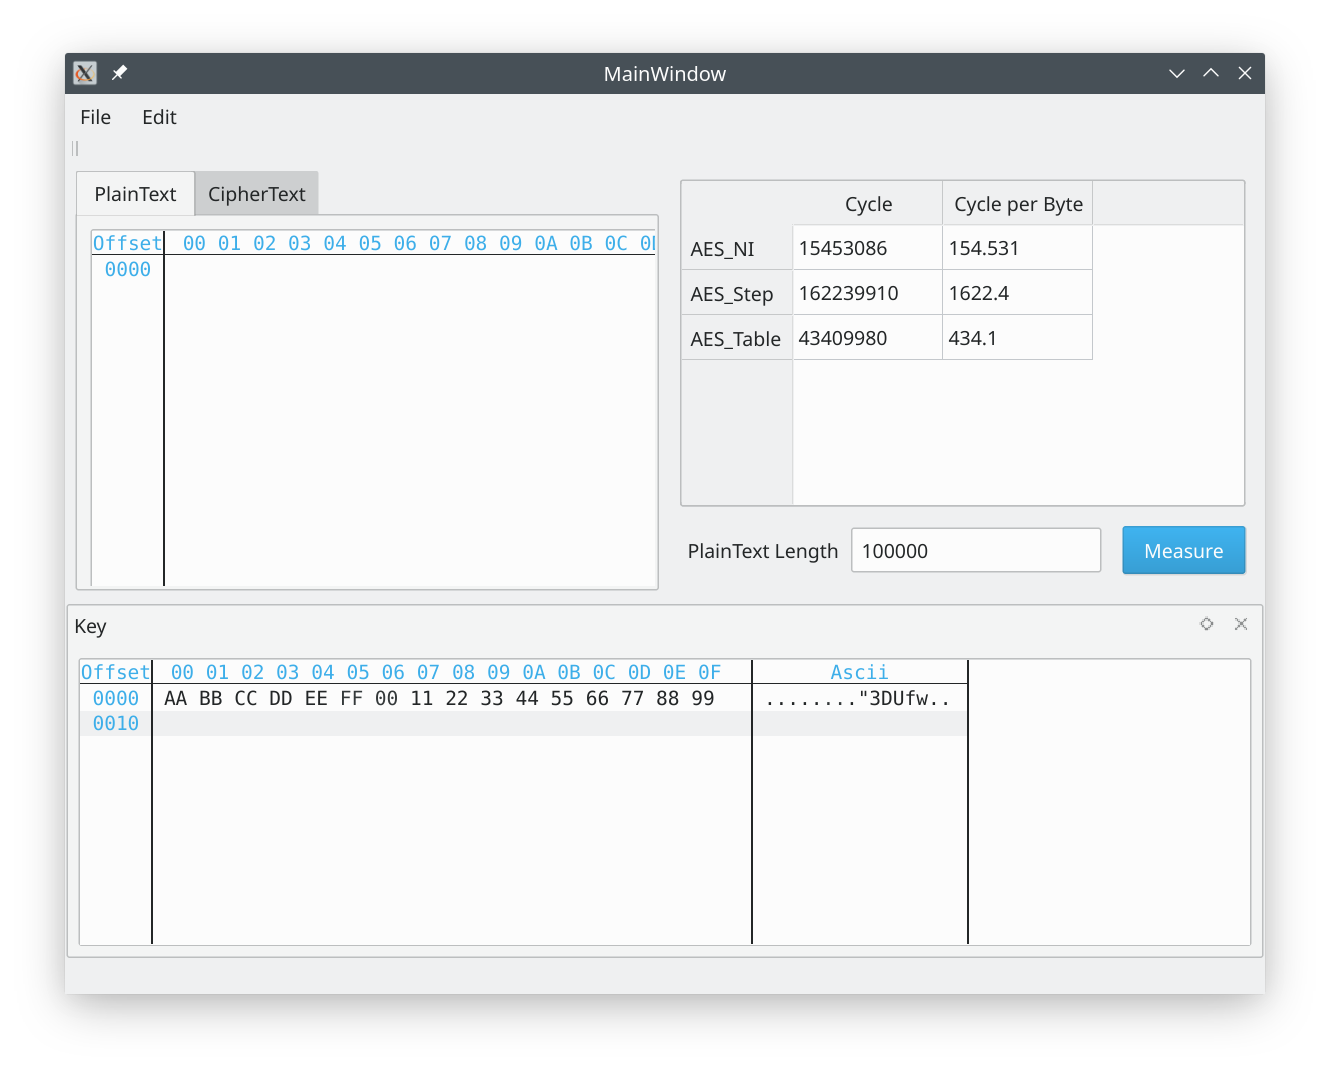
\includegraphics[width = 0.45\textwidth]{Debug.png}
	}
	\subfigure[Release] {
	\label{Release Test}
	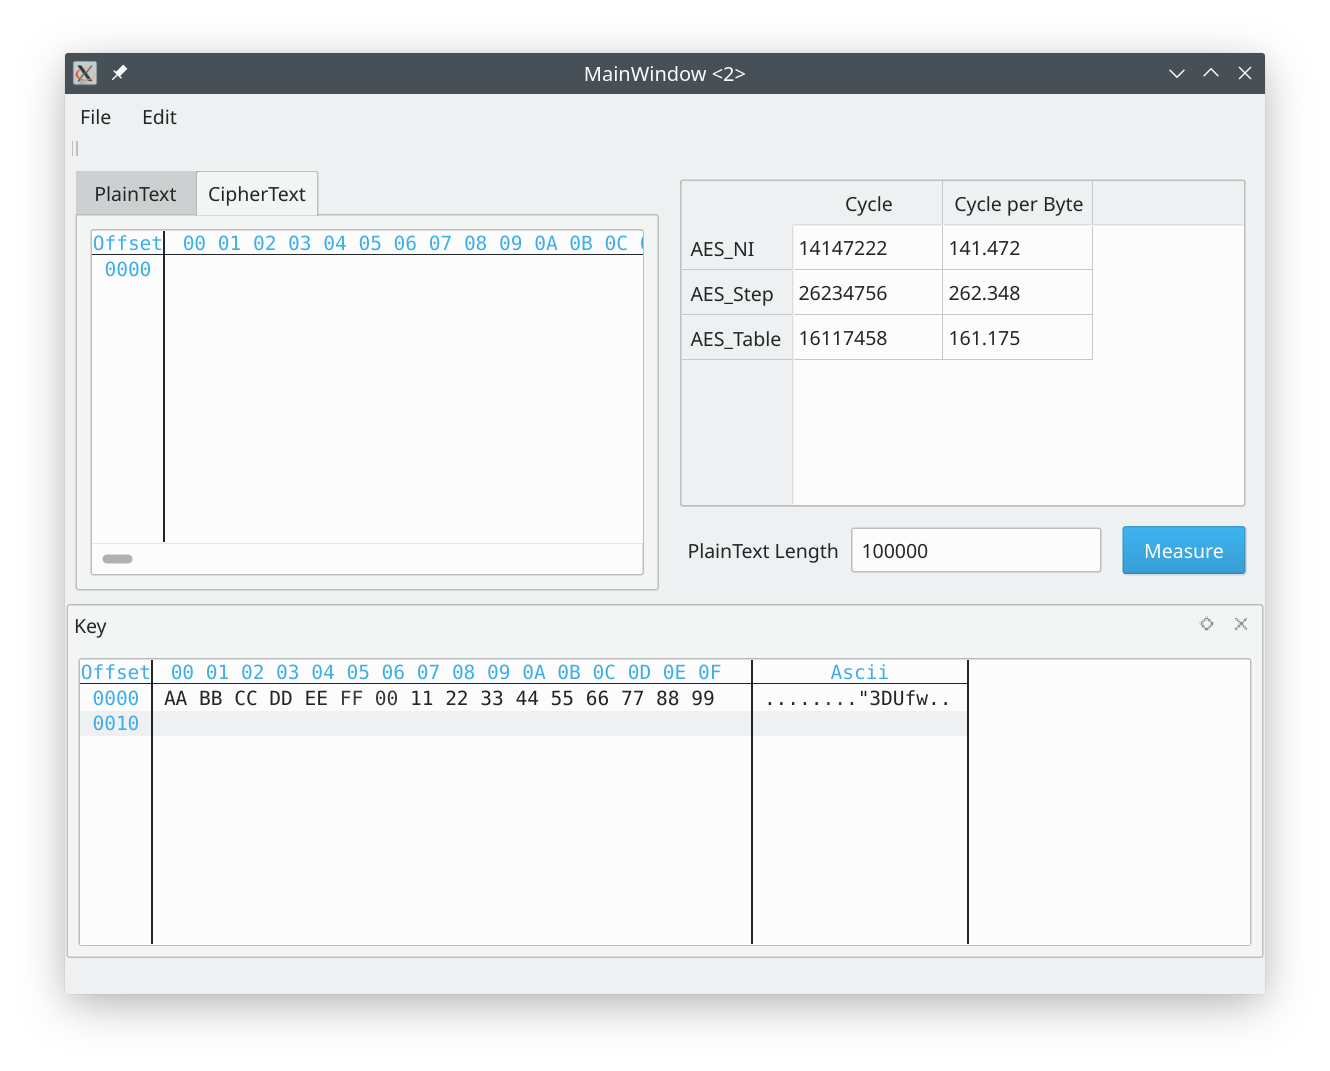
\includegraphics[width = 0.45\textwidth]{Release.png}
	}
    \caption{Test}
\end{figure}
如图\ref{Debug Test}所示,在Debug模式下,加密任意长度为100000 byte的随机字符串的测试中,AES\_NI 实现的的效率为\textbf{154.531 cycles/byte},效率约为一般实现AES\_Step(\textbf{1622.4 cycles/byte})的十倍。而查表法实现AES\_Table的效率为\textbf{434.1 cycles/byte},也显著高于一般实现。

在Release模式下的测试结果如图\ref{Release Test}所示,在良好的编译优化下,三者之间的效率差距被大大缩小,但AES\_NI与一般实现之间仍存在约2倍的差距。注意到AES\_NI的效率并没有进一步提高,猜测可能是编译优化中对另外两种实现采用了向量化操作,从而将其效率提升到了与AES\_NI相近的水平。
\section{讨论}
	采用面向对象的设计,对算法进行了封装,但没有进一步测量对象构造的开销是否对加密效率存在显著影响,若需执行进一步更加严谨的测量,需要考虑到扣除这一部分的代价。


\end{CJK}
\end{document}
